\chapter{Introducción}
\label{ch:introduccion}
\chapterminitoc

% El presente capítulo establece los fundamentos físicos que rigen la dinámica de los
% pulsos láser ultrarrápidos. A partir de estos conceptos, se formaliza el problema de optimi-
% zación multidimensional inherente al control coherente de dichos pulsos. Finalmente, se
% introduce el aprendizaje automático (machine learning) como un marco computacional
% avanzado para abordar esta complejidad, ofreciendo una perspectiva actualizada del estado
% del arte. Este documento forma parte de un artículo de revisión actualmente en preparación.

Esta tesis estudia cómo optimizar de manera automática los parámetros de un láser ultrarrápido para que genere el pulso deseado. El presente capítulo enmarca ese problema y delimita el trabajo. Comienza situando a los láseres ultrarrápidos y su relevancia científica y tecnológica; muestra a continuación por qué controlar el pulso equivale a resolver un problema de optimización de alta dimensión que los métodos de ajuste tradicionales no afrontan de manera satisfactoria; y, sobre ese diagnóstico, formula la pregunta de investigación, los objetivos, las hipótesis y el alcance del estudio, así como el aporte que la tesis realiza al campo. El tratamiento es deliberadamente conceptual: los fundamentos físicos y computacionales que sostienen el argumento se desarrollan con detalle en el marco teórico (Capítulo~\ref{ch:Theoretical background}). El capítulo concluye con un mapa de lectura del resto del documento.

\section{Contexto y relevancia de los láseres ultrarrápidos}
\label{sec:contexto-relevancia}
 
Pocos instrumentos han ampliado tanto el horizonte de lo observable como el láser ultrarrápido. Su rasgo definitorio es la brevedad: emite pulsos de luz cuya duración se mide en femtosegundos ($10^{-15}$~s) e incluso en attosegundos ($10^{-18}$~s), escalas tan ajenas a la experiencia cotidiana que la proporción entre un attosegundo y un segundo es comparable a la que existe entre un segundo y la edad del universo. Esa brevedad es justamente lo que los hace valiosos: un pulso más corto que el tiempo característico de un proceso permite congelarlo y seguirlo, de modo que la dinámica de electrones, átomos y moléculas (antes inaccesible por ser demasiado rápida) queda al alcance de la medición directa. La Figura~\ref{fig:escala-tiempo} sitúa estas escalas temporales junto con los procesos físicos y las técnicas láser asociadas a cada una.

\begin{figure}[t]
  \centering
  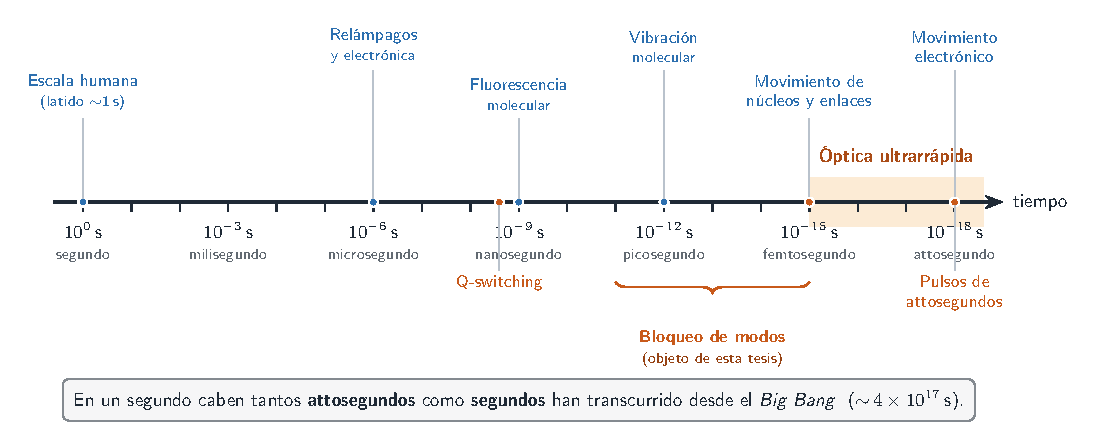
\includegraphics[width=\textwidth]{chapters/images/ch1/fig_escala_tiempo.pdf}
  \caption[Escala de tiempos de la física ultrarrápida]{Escala de tiempos de la
    física ultrarrápida, en eje logarítmico. Sobre el eje se señalan procesos
    físicos característicos de cada escala —desde la escala humana hasta el
    movimiento electrónico— y, bajo él, las técnicas de generación de pulsos
    láser: el \emph{Q-switching}, el bloqueo de modos (objeto de esta tesis) y la
    generación de pulsos de attosegundos. La ventana de la óptica ultrarrápida,
    entre femtosegundos y attosegundos, aparece resaltada.}
  \label{fig:escala-tiempo}
\end{figure}
  
La madurez e impacto de este campo quedaron consagrados con el Premio Nobel de Física de 2023, otorgado a Pierre Agostini, Ferenc Krausz y Anne L'Huillier por el desarrollo de métodos experimentales capaces de generar pulsos de luz de attosegundos, un hito que abrió la puerta a observar el movimiento de los electrones dentro de la materia \cite{Nobel2023}. Ese reconocimiento corona una trayectoria de varias décadas de progreso en la generación y el control de pulsos cada vez más breves e intensos, sostenida por avances sucesivos en medios de ganancia de banda ancha y en arquitecturas de oscilador y amplificación \cite{Krausz1992,Keller2022}.
 
El valor de los láseres ultrarrápidos se manifiesta en un abanico de aplicaciones que atraviesa la ciencia y la tecnología. Su resolución temporal extrema los convierte en el estroboscopio de la espectroscopía de bombeo-sonda, con la que se sigue en tiempo real la relajación electrónica y las transiciones de fase ultrarrápidas. Su capacidad de confinar intensidad en volúmenes microscópicos sustenta técnicas de biofotónica como la microscopía de excitación multifotónica, que permite obtener imágenes tridimensionales de tejido vivo. Su amplísimo ancho de banda es la base de los peines de frecuencia ópticos, que enlazan los dominios del tiempo y la frecuencia con precisión metrológica. Y su elevadísima intensidad pico (accesible gracias a la amplificación de pulsos chirpeados \cite{StricklandMourou1985}) habilita desde la física de campos extremos hasta el micromaquinado de materiales en régimen de ablación en frío. La consolidación de fuentes compactas y fiables, en estado sólido y en fibra, ha extendido este repertorio del laboratorio especializado a un número creciente de entornos \cite{FermannHartl2013}.
 
Conviene, sin embargo, no perder de vista de dónde proviene cada uno de esos pulsos. Detrás de toda esta versatilidad hay siempre un oscilador láser: una cavidad en la que el pulso se forma, se moldea y se estabiliza vuelta tras vuelta. Las propiedades que cada aplicación explota (la duración, la energía, la estabilidad del tren de pulsos) no son un dato de partida, sino el resultado de la dinámica interna de esa cavidad y del modo en que se la ajusta. Es ahí, en el gobierno de la cavidad, donde se decide la calidad del pulso, y es ahí donde surge el problema que esta tesis aborda.


\section{El problema del control y la optimización de parámetros}
\label{sec:problema-control}
 
Disponer de una fuente capaz de emitir pulsos ultracortos no equivale, por sí solo, a disponer del pulso que cada aplicación requiere. Encender el oscilador y obtener un tren de pulsos con una duración, una energía y una estabilidad prescritas son dos cosas distintas: lo segundo exige situar la cavidad en un punto de operación muy concreto, definido por el ajuste simultáneo de un conjunto de magnitudes de control. Es en ese tránsito (de la mera capacidad de generar luz pulsada al gobierno fino de sus propiedades) donde aparece el problema que esta tesis aborda.

\begin{figure}[t]
  \centering
  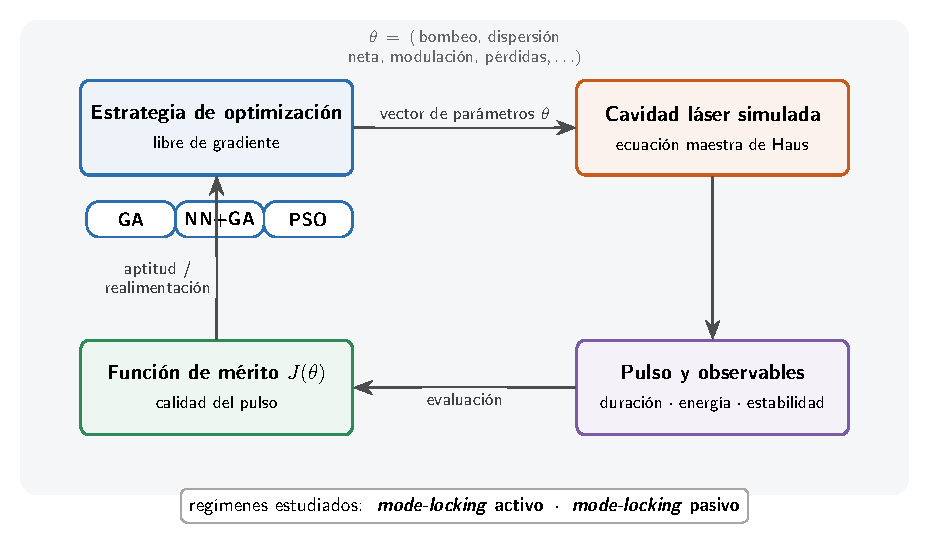
\includegraphics[width=0.92\textwidth]{chapters/images/ch1/fig_esquema_optimizacion.pdf}
  \caption[Ciclo de optimización de la cavidad láser]{Esquema conceptual del
    ciclo de optimización de la cavidad láser. Cada estrategia de optimización
    libre de gradiente (GA, NN+GA o PSO) propone un vector de parámetros
    $\theta$ (bombeo, dispersión neta, modulación, pérdidas, entre otros) que la
    cavidad simulada, modelada por la ecuación maestra de Haus, transforma en un
    pulso. Los observables del pulso (duración, energía y estabilidad) definen la
    función de mérito $J(\theta)$, que realimenta a la estrategia de búsqueda. El
    estudio compara los tres métodos en los regímenes de \emph{mode-locking}
    activo y pasivo.}
  \label{fig:ciclo-optimizacion}
\end{figure}
 
El estado de la cavidad, y con él la existencia misma del pulso y sus características, queda determinado por un puñado de parámetros accesibles al operador: la potencia de bombeo, que fija la ganancia disponible; los parámetros del elemento que produce el anclaje de modos (profundidad y frecuencia de modulación en el régimen activo, profundidad de modulación y tiempo de relajación del absorbente saturable en el pasivo); la dispersión intracavidad neta; el ancho de banda del filtrado espectral; y el acoplamiento de salida, entre otros \cite{Haus2000,Keller2022}. Gobernar el pulso equivale, así, a elegir un punto dentro de un espacio de parámetros de varias dimensiones. La pregunta operativa de toda la tesis puede enunciarse en estos términos: ¿qué combinación de esos valores produce el pulso deseado?
 
La dificultad no reside en el número de variables, sino en que no son independientes. El pulso \emph{mode-locked} es el resultado de un equilibrio delicado entre efectos físicos opuestos (dispersión frente a no linealidad, ganancia frente a pérdidas), de modo que perturbar un solo parámetro rompe ese equilibrio y obliga a reajustar los demás para preservar la estabilidad del pulso. El sistema no admite, por tanto, una optimización variable por variable: los grados de libertad están acoplados, y el efecto de cada uno depende del valor de todos los otros. La descripción formal de ese acoplamiento (la dinámica de la envolvente en la cavidad y el balance que sostiene al pulso) corresponde al marco teórico y se desarrolla en el Capítulo~\ref{ch:Theoretical background}; aquí basta con retener su consecuencia: el ajuste es un problema global, no una suma de ajustes locales.
 
Ese acoplamiento dota al espacio de búsqueda de una estructura particularmente hostil. Es un espacio de \emph{alta dimensión}, en el que el volumen a explorar crece de forma explosiva con cada grado de libertad añadido; es \emph{no convexo}, poblado de óptimos locales en los que los métodos basados en gradiente quedan atrapados; y es \emph{multiestable}, en el sentido de que para un mismo conjunto de parámetros pueden coexistir varios regímenes de operación estables (onda continua, anclaje fundamental y armónico, regímenes multipulso o de \emph{Q-switching}), de manera que el estado finalmente alcanzado depende no solo de dónde se está en el espacio, sino del camino por el que se llegó \cite{Andral2015,GreluAkhmediev2012,Kokhanovskiy2022}. A ello se añaden las transiciones abruptas entre regímenes y el ruido inherente a cualquier oscilador real, que exigen que una solución útil no sea solo óptima en un punto, sino además robusta frente a perturbaciones.
 
El cuadro resultante es el de un problema de optimización de caja negra: no se dispone de una expresión cerrada que relacione los parámetros con la calidad del pulso, cada evaluación obliga a propagar el estado de la cavidad hasta su régimen estacionario, y el paisaje de búsqueda carece de la regularidad que los métodos analíticos requieren \cite{Genty2021,Woodward2016}. Optimizar un láser ultrarrápido es, en definitiva, un problema de búsqueda en un espacio difícil, no un cálculo que pueda resolverse de forma cerrada. Este es el obstáculo central que motiva la presente tesis; antes de presentar las estrategias que la comunidad ha desarrollado para sortearlo, conviene examinar por qué los enfoques de ajuste tradicionales resultan insuficientes frente a un espacio con estas características. La Figura~\ref{fig:ciclo-optimizacion} resume el ciclo de optimización que de aquí resulta y que esta tesis aborda: una estrategia de búsqueda —en este trabajo, el algoritmo genético (GA), su acoplamiento con una red neuronal (NN+GA) y la optimización por enjambre de partículas (PSO)— propone vectores de parámetros que la cavidad simulada convierte en pulsos, cuya calidad, cuantificada por una función de mérito, realimenta la búsqueda.


\section{Limitaciones de los enfoques tradicionales de ajuste}
\label{sec:enfoques-tradicionales-intro}
 
Frente a un espacio de búsqueda con las características descritas, las estrategias con que tradicionalmente se ha ajustado un láser \emph{mode-locked} resultan insuficientes, cada una por una razón distinta. El enfoque históricamente dominante ha sido el \emph{ajuste manual experto}: un operador modifica iterativamente los parámetros accesibles mientras vigila la traza temporal y el espectro, guiándose por heurísticas adquiridas con la práctica. Su fortaleza es la intuición acumulada, pero sus límites son estructurales: es lento, porque explora el espacio punto a punto; es poco reproducible, porque el resultado depende del operador; no escala con la dimensión; y no ofrece recuperación automática cuando la deriva ambiental saca al láser de su régimen \cite{Pu2019,Pu2020}.
 
La alternativa de fuerza bruta (el \emph{barrido exhaustivo} del espacio de parámetros) garantiza cobertura y reproducibilidad, pero choca con la maldición de la dimensión: el número de evaluaciones crece exponencialmente y, como cada una exige llevar la cavidad a su estado estacionario, el costo se vuelve prohibitivo ya para pocas variables \cite{Andral2015}. El \emph{diseño analítico} basado en la teoría de cavidad ofrece, por su parte, leyes de escala y valores de partida útiles, pero su validez descansa en aproximaciones que eluden justamente los fenómenos que dominan el problema real (multiestabilidad, transiciones abruptas y ruido), de modo que entrega un buen punto inicial, no una solución en lazo cerrado. Y los métodos de \emph{control clásico} y de \emph{optimización basada en gradiente} presuponen una respuesta suave y diferenciable entre la acción y el observable, hipótesis que una cavidad multiestable e histerética incumple de raíz \cite{Kokhanovskiy2022}.
 
El denominador común es que ninguno de estos enfoques afronta de manera conjunta las dificultades del problema: explorar globalmente un espacio de alta dimensión y no convexo, tolerar su naturaleza de caja negra y discontinua, y operar de forma autónoma y robusta frente al ruido. Es precisamente esa carencia simultánea la que define el nicho ocupado, en la última década, por los algoritmos de optimización inspirados en la naturaleza y las técnicas de aprendizaje automático \cite{Genty2021}: métodos que no exigen gradientes, exploran soluciones en paralelo y se prestan a automatizar el ciclo completo de ajuste. La revisión sistemática de cómo el campo ha desplegado esas herramientas (y de las brechas que deja abiertas) constituye el Estado del Arte que se presenta en el Capítulo~\ref{ch:estado del arte}.


\section{Planteamiento del problema y pregunta de investigación}
\label{sec:planteamiento}
 
Las secciones anteriores permiten enunciar el problema con precisión. Generar el pulso que una aplicación requiere equivale a fijar la configuración de parámetros de un oscilador láser, y ese ajuste constituye un problema de optimización de caja negra (de alta dimensión, no convexo, multiestable y ruidoso) frente al cual los enfoques tradicionales de ajuste resultan insuficientes. La comunidad ha respondido adoptando algoritmos de optimización inspirados en la naturaleza y técnicas de aprendizaje automático, capaces de explorar globalmente el espacio sin exigir gradientes ni un modelo analítico de la respuesta de la cavidad. Sin embargo, como se documenta en el Estado del Arte (Capítulo~\ref{ch:estado del arte}), ese cuerpo de trabajo deja dos vacíos persistentes: por un lado, la optimización automatizada se ha concentrado casi por completo en el \emph{mode-locking} pasivo, dejando el régimen activo notablemente subexplorado \cite{KuizengaSiegman1970}; por otro, la literatura está organizada como una colección de estudios de caso aislados, sin comparaciones sistemáticas que mantengan fijos el láser, el espacio de parámetros y la función objetivo para variar únicamente el algoritmo \cite{Genty2021,Jiang2022}.
 
De esos dos vacíos surge la pregunta que vertebra esta tesis: \emph{¿cómo se comparan tres estrategias de optimización inspiradas en la naturaleza (el algoritmo genético (GA), una red neuronal acoplada al algoritmo genético como sustituto del simulador (NN+GA) y la optimización por enjambre de partículas (PSO)) al ajustar los parámetros de una cavidad láser ultrarrápida, evaluadas bajo idénticas condiciones de simulación numérica y en los regímenes de} mode-locking \emph{tanto activo como pasivo?} La pregunta se descompone en tres interrogantes operativos: qué calidad de pulso alcanza cada método respecto a una misma función de mérito; a qué costo computacional lo hace (en número de evaluaciones del simulador y en tiempo hasta la convergencia); y con qué robustez reproduce su desempeño al variar las condiciones iniciales y la modalidad de anclaje.
 
El interés de la pregunta no es solo práctico sino metodológico. Las tres estrategias comparten el paradigma de la optimización libre de gradiente, pero difieren de manera controlada en la mecánica de búsqueda y en el modo de evaluar la función objetivo, de suerte que confrontarlas sobre un mismo banco de pruebas permite atribuir las diferencias de rendimiento al método y no a las particularidades del problema. Responderla, además, sobre las dos modalidades de \emph{mode-locking} aborda simultáneamente las dos brechas señaladas. Los objetivos que concretan esta pregunta en entregables verificables se enuncian a continuación.


\section{Objetivos}
\label{sec:objetivos}
 
\subsection*{Objetivo general}
 
Comparar de forma sistemática tres estrategias de optimización inspiradas en la naturaleza (el algoritmo genético (GA), una red neuronal acoplada al algoritmo genético como sustituto del simulador (NN+GA) y la optimización por enjambre de partículas (PSO)) en el ajuste de los parámetros de una cavidad láser ultrarrápida simulada numéricamente, evaluándolas bajo idénticas condiciones en los regímenes de \emph{mode-locking} activo y pasivo.
 
\subsection*{Objetivos específicos}
 
\begin{enumerate}
  \item Implementar un modelo numérico de la cavidad láser, basado en la ecuación maestra de Haus, capaz de reproducir los regímenes de operación conocidos y de servir como entorno de evaluación para los algoritmos de optimización.
 
  \item Formular el problema de optimización asociado, definiendo las variables de decisión, sus rangos y restricciones, y una función de mérito que cuantifique la calidad del pulso a partir de observables del estado estacionario de la cavidad.
 
  \item Implementar y ajustar un algoritmo genético sobre ese problema, que sirva como línea base de referencia frente a la cual contrastar las demás estrategias.
 
  \item Construir una red neuronal que actúe como sustituto (\emph{surrogate}) del simulador y acoplarla al algoritmo genético (NN+GA), con el fin de reducir el número de evaluaciones costosas durante la búsqueda.
 
  \item Implementar la optimización por enjambre de partículas sobre el mismo problema, con su propia parametrización del proceso de búsqueda.
 
  \item Comparar los tres métodos en los regímenes de \emph{mode-locking} activo y pasivo bajo un conjunto común de métricas (calidad del pulso, costo computacional y robustez), de modo que las diferencias de desempeño puedan atribuirse al algoritmo y no a las particularidades del problema.
\end{enumerate}
 
Cada objetivo específico se traduce en un componente verificable del trabajo: los dos primeros definen el entorno de simulación y el problema de optimización (Capítulo~\ref{ch:Theoretical background} y Capítulo~\ref{ch:Methodology}); el tercero, el cuarto y el quinto, la implementación de cada método; y el sexto, el estudio comparativo que constituye el aporte central de la tesis y que se desarrolla en los capítulos de metodología y resultados.

 
\section{Hipótesis, alcance y limitaciones}
\label{sec:hipotesis-alcance}
 
La hipótesis de trabajo que orienta este estudio es que las tres estrategias consideradas son capaces de alcanzar soluciones de calidad comparable sobre la misma función de mérito, pero difieren de manera medible en su eficiencia y su comportamiento de búsqueda (en el número de evaluaciones del simulador que requieren, en el tiempo hasta la convergencia y en la robustez de su desempeño), de modo que existe un método preferible según el régimen de \emph{mode-locking} considerado. En particular, se espera que el acoplamiento de la red neuronal como sustituto del simulador (NN+GA) reduzca el costo de evaluación frente al algoritmo genético puro, y que la estructura más determinista y de menor dimensión del régimen activo favorezca una convergencia más rápida que la del régimen pasivo. El estudio comparativo está diseñado para confirmar o refutar estas expectativas sobre una base empírica controlada.
 
El alcance del trabajo queda delimitado por tres decisiones. Primero, el estudio se realiza enteramente en \emph{simulación numérica}: la cavidad se representa mediante el modelo de la ecuación maestra de Haus, que actúa como entorno de evaluación para los optimizadores. Segundo, la comparación abarca las dos modalidades de \emph{mode-locking}, activa y pasiva, y se restringe a las tres estrategias seleccionadas (GA, NN+GA y PSO), elegidas por compartir el paradigma de la optimización libre de gradiente y diferir de forma controlada en la mecánica de búsqueda. Tercero, la calidad de las soluciones se mide mediante una función de mérito definida sobre observables del pulso (duración, energía y estabilidad) en el estado estacionario de la cavidad.
 
De ese alcance se derivan sus limitaciones, que conviene reconocer explícitamente. Al emplear simulación pura como generador de datos, los resultados no incorporan de forma plena el ruido, la deriva de parámetros y las no idealidades presentes en un montaje experimental, por lo que sus conclusiones se circunscriben al modelo y no se extrapolan sin más a un laboratorio \cite{Baumeister2018}. Del mismo modo, el desempeño observado depende del modelo de cavidad adoptado y de los rangos de parámetros explorados, cuya elección acota el espacio de búsqueda. Finalmente, el trabajo se concentra en la familia de optimizadores libres de gradiente y deja fuera de su foco comparativo el aprendizaje por refuerzo profundo, que —pese a su potencial para el control de la multiestabilidad \cite{Kokhanovskiy2024}— se considera un horizonte de extensión y no parte del estudio comparativo. Estas limitaciones no debilitan el aporte: lo delimitan con honestidad y orientan la interpretación de los resultados.

\section{Aporte de la tesis}
\label{sec:aporte}
 
La contribución de esta tesis se define por las dos brechas que el Estado del Arte deja al descubierto y que el trabajo aborda de manera conjunta en un único diseño experimental. La primera es una brecha de \emph{objeto}. La optimización automatizada de láseres \emph{mode-locked} se ha desarrollado casi exclusivamente sobre el régimen pasivo, dejando el \emph{mode-locking} activo notablemente subexplorado como problema de ajuste inteligente \cite{Woodward2016,Andral2015}. Esta tesis amplía ese alcance al aplicar un mismo conjunto de optimizadores a ambas modalidades, lo que permite examinar si las técnicas que han demostrado su eficacia en el régimen pasivo conservan su desempeño cuando se enfrentan a la dinámica más determinista y de menor dimensión del activo.
 
La segunda es una brecha de \emph{método}. La literatura está organizada como una colección de estudios de caso en los que cada trabajo valida un único algoritmo sobre un único problema, lo que impide atribuir limpiamente las diferencias de rendimiento al método empleado \cite{Genty2021}. El aporte de esta tesis es un estudio comparativo controlado de GA, NN+GA y PSO que mantiene fijos el láser, el espacio de parámetros y la función de mérito, y varía únicamente el algoritmo de optimización, de modo que las diferencias observadas reflejen el comportamiento del método y no las particularidades del problema. Atender ambas brechas en un mismo diseño (los tres optimizadores sobre las dos modalidades de anclaje) es lo que distingue a este trabajo de los antecedentes revisados.
 
A esas dos contribuciones se añade un valor metodológico transversal: el estudio se articula como un protocolo comparativo \emph{reproducible}, con un mismo simulador, un mismo conjunto de métricas (calidad del pulso, costo computacional y robustez) y un control explícito de la aleatoriedad y de las repeticiones. Más allá de los resultados concretos que arroje, ese protocolo constituye un marco con el que futuros métodos de optimización podrán evaluarse sobre una base común, lo que responde directamente a la fragmentación que caracteriza al campo.


\section{Resumen de contenido}
\label{sec:estructura-documento}
 
El resto de la tesis sigue el mismo hilo conductor que esta introducción, avanzando de la caracterización del problema a su resolución y a la interpretación de los resultados. El Capítulo~\ref{ch:estado del arte} presenta el estado del arte: revisa la literatura sobre optimización de láseres ultrarrápidos siguiendo un recorrido que va de la física de la cavidad a las estrategias computacionales, y justifica, sobre esa base, las dos brechas que el trabajo se propone llenar. El Capítulo~\ref{ch:Theoretical background} desarrolla el marco teórico, reuniendo las herramientas físicas y computacionales necesarias para el resto del documento: la dinámica de la cavidad y la ecuación maestra de Haus, los regímenes de \emph{mode-locking} activo y pasivo, y los fundamentos de las tres estrategias de optimización.
 
El Capítulo~\ref{ch:Methodology} expone la metodología del estudio comparativo: el modelo numérico de la cavidad, la definición del problema de optimización y de la función de mérito, la implementación de cada método y el diseño del experimento que los enfrenta bajo idénticas condiciones. El capítulo de resultados presenta los hallazgos (la validación del modelo y el desempeño de cada estrategia en ambas modalidades de anclaje) sin interpretarlos todavía. El capítulo de discusión da sentido a esos resultados, interpreta físicamente las soluciones halladas, contrasta las fortalezas y debilidades de cada método y dialoga con la literatura revisada. Finalmente, el capítulo de conclusiones cierra el círculo abierto en esta introducción: responde a la pregunta de investigación, recapitula las contribuciones y señala las líneas de trabajo futuro, entre ellas la validación experimental y la extensión al aprendizaje por refuerzo.